% OpenMP для разных стратегий распараллеливания для Римановского решателя.
\subsection{Исследование масштаибруемости плотных параллельных вычислений на микропроцессорах Intel}

На рис. 1 представлены графики ускорения скалярной версии римановского решателя при увеличении количества потоков с 1 до 160.
Для каждого вычислительного узла явно просматриваются отрезки квазилинейного ускорения, которые завершаются заметными провалами.
Длина этих отрезков во всех случаях равняется суммарному количеству ядер в узле, а провалы обусловлены конфликтами за аппаратные ресурсы.
При этом стоит отметить, что хоть максимальное количество доступных потоков для вычислительного узла на базе микропроцессора KNL равняется 288, однако на графике не показаны значения больше 160, так как сверх этого значения наблюдается только деградация производительности, и наиболее эффективное использование зафиксировано в диапазоне потоков 140-144.
Также можно отметить, что для всех микропроцессоров ускорение близко к линейному до тех пор, пока каждый поток запущен на своем отдельном ядре.

\begin{figure}[ht]
\centering
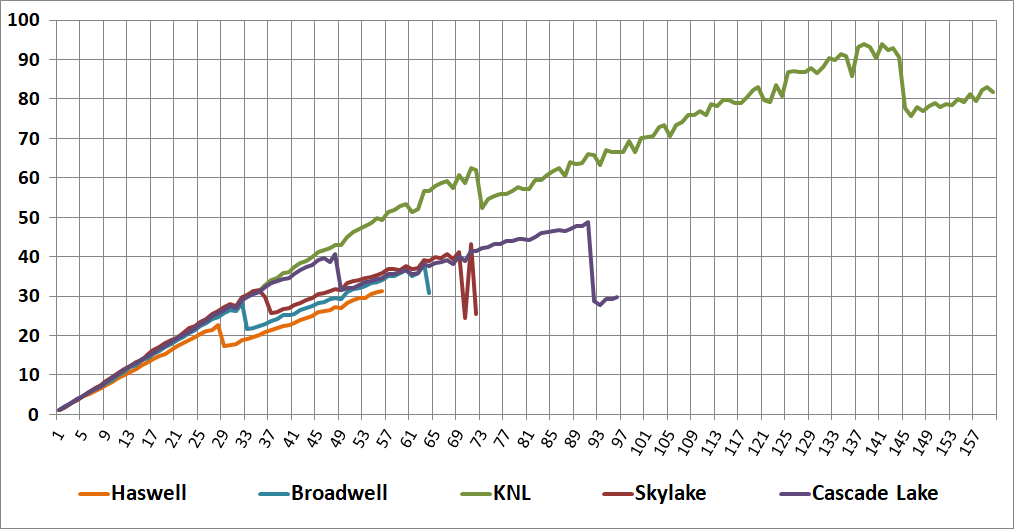
\includegraphics[width=0.4\textwidth]{./pics/text_3_omp2/speedup_scalar.png}
\singlespacing
\captionstyle{center}\caption{График ускорения скалярной версии римановского решателя для микропроцессоров Haswell, Broadwell, KNL, Skylake, Cascade Lake для количества потоков от 1 до 160.}
\label{fig:text_3_omp2_speedup_scalar}
\end{figure}

\begin{figure}[ht]
\centering
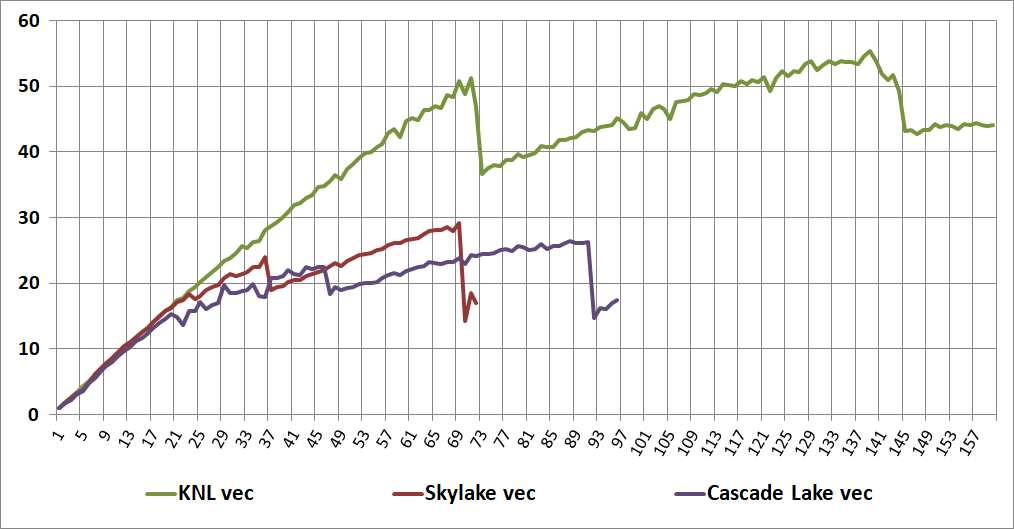
\includegraphics[width=0.4\textwidth]{./pics/text_3_omp2/speedup_vec.png}
\singlespacing
\captionstyle{center}\caption{График ускорения векторизованной версии римановского решателя для микропроцессоров KNL, Skylake, Cascade Lake для количества потоков от 1 до 160.}
\label{fig:text_3_omp2_speedup_vec}
\end{figure}

На рис. 2 представлены аналогичные данные, но уже для векторизованной версии римановского решателя (соответственно только для микропроцессоров KNL, Skylake, Cascade Lake).
Из графиков видно, что характер ускорения для KNL практически не поменялся, тогда как Skylake и Cascade Lake демонстрируют серьезную деградацию ускорения вычислений уже на небольшом количестве потоков.

\begin{figure}[ht]
\centering
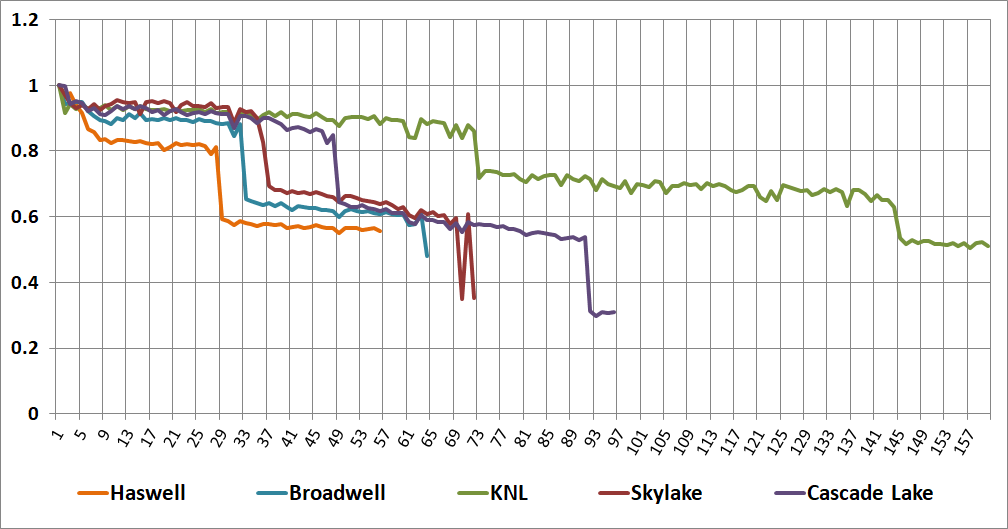
\includegraphics[width=0.4\textwidth]{./pics/text_3_omp2/eff_scalar.png}
\singlespacing
\captionstyle{center}\caption{График масштабируемости скалярной версии римановского решателя для микропроцессоров Haswell, Broadwell, KNL, Skylake, Cascade Lake для количества потоков от 1 до 160.}
\label{fig:text_3_omp2_eff_scalar}
\end{figure}

\begin{figure}[ht]
\centering
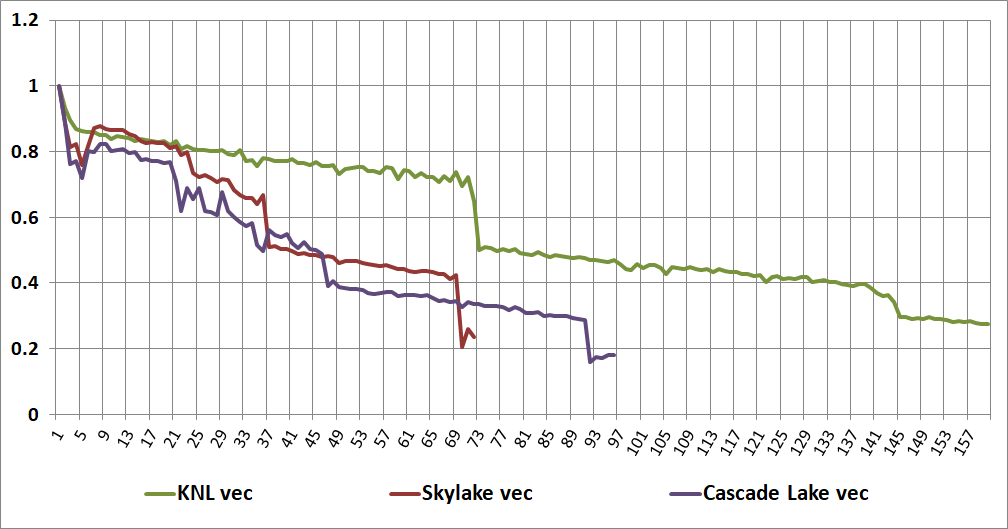
\includegraphics[width=0.4\textwidth]{./pics/text_3_omp2/eff_vec}
\singlespacing
\captionstyle{center}\caption{График масштабируемости векторизованной версии римановского решателя для микропроцессоров KNL, Skylake, Cascade Lake для количества потоков от 1 до 160.}
\label{fig:text_3_omp2_eff_scalar}
\end{figure}

На рис. 3 и рис. 4 приведены данные показателей эффективности масштабирования римановского решателя (скалярной и векторизованной версии соответственно).
Данные иллюстрации более информативные.
Например, из рис. 3 видно, что масштабируемость при количестве потоков, не превышающем количество ядер вычислительного узла, находится для всех микропроцессоров на хорошем уровне в диапазоне 0,8 - 1,0.
Рис. 4 наглядно демонстрирует хорошую масштабируемость векторизованного римановского решателя для микропроцессора KNL с показателем, близким к 0,8 вплоть до использования 72 потоков, тогда как узлы на базе микропроцессоров Skylake и Cascade Lake деградируют на масштабировании векторизованной версии римановского решателя на достаточно небольшом количестве потоков.
